% !TEX root = ../praca_inzynierska.tex
\section{Uczenie ze wzmocnieniem w grach komputerowych}
\label{sec:rl-gry}

\subsection{Podstawy uczenia ze wzmocnieniem}
\label{subsec:podstawy-rl}

Uczenie ze wzmocnieniem jest dziedziną uczenia maszynowego, w której agent uczy się podejmować sekwencje decyzji na podstawie interakcji ze środowiskiem \cite{sutton2018}. W odróżnieniu od uczenia nadzorowanego agent nie otrzymuje przykładów poprawnych odpowiedzi. Jedyną informacją zwrotną jest skalarna nagroda, którą środowisko przekazuje po każdej wykonanej akcji. Celem agenta jest takie dobieranie akcji, aby suma nagród uzyskanych w długim horyzoncie czasowym była jak największa.

Interakcja przebiega w dyskretnych krokach czasowych $t = 0, 1, 2, \ldots$ W każdym kroku agent obserwuje stan środowiska $s_t$, wybiera akcję $a_t$, a środowisko odpowiada nagrodą $r_{t+1}$ oraz nowym stanem $s_{t+1}$. Schemat ten powtarza się aż do osiągnięcia stanu terminalnego, który kończy epizod.

\subsubsection{Proces decyzyjny Markowa}

Formalnym modelem środowiska w uczeniu ze wzmocnieniem jest proces decyzyjny Markowa (ang. \emph{Markov decision process}, MDP). Zgodnie ze wzorem \eqref{eq:mdp} opisuje go krotka pięciu elementów \cite{sutton2018}:
\begin{equation}
	\mathcal{M} = (\mathcal{S}, \mathcal{A}, P, R, \gamma),
	\label{eq:mdp}
\end{equation}
gdzie: $\mathcal{S}$ -- zbiór stanów, $\mathcal{A}$ -- zbiór akcji, $P(s' \mid s, a)$ -- prawdopodobieństwo przejścia do stanu $s'$ po wykonaniu akcji $a$ w stanie $s$, $R(s, a)$ -- oczekiwana nagroda za wykonanie akcji $a$ w stanie $s$, $\gamma \in [0, 1)$ -- współczynnik dyskontowania.

Nazwa procesu pochodzi od własności Markowa: następny stan zależy wyłącznie od stanu bieżącego i wybranej akcji, a nie od całej wcześniejszej historii. W praktyce oznacza to, że stan musi zawierać wszystkie informacje potrzebne do podjęcia decyzji.

W grze Snake rozważanej w niniejszej pracy elementy krotki \eqref{eq:mdp} mają następującą interpretację:
\begin{itemize}
	\item stan $s_t$ to wektor 11 cech binarnych opisujących zagrożenia wokół głowy węża, kierunek ruchu i położenie jedzenia (szczegóły w rozdziale \ref{sec:projekt}),
	\item zbiór akcji $\mathcal{A} = \{\text{prosto}, \text{w prawo}, \text{w lewo}\}$ zawiera skręty względem bieżącego kierunku ruchu,
	\item nagroda wynosi $+10$ za zjedzenie pożywienia, $-10$ za kolizję oraz $\pm 0{,}1$ za zbliżenie się do pożywienia lub oddalenie od niego,
	\item epizod kończy się kolizją ze ścianą lub z ciałem węża.
\end{itemize}

\subsubsection{Zwrot i współczynnik dyskontowania}

Miarą jakości zachowania agenta od chwili $t$ jest zwrot (ang. \emph{return}), czyli zdyskontowana suma przyszłych nagród, określona wzorem \eqref{eq:zwrot}:
\begin{equation}
	G_t = r_{t+1} + \gamma r_{t+2} + \gamma^2 r_{t+3} + \ldots = \sum_{k=0}^{\infty} \gamma^k r_{t+k+1}.
	\label{eq:zwrot}
\end{equation}

Występujący we wzorze \eqref{eq:zwrot} współczynnik $\gamma$ określa, jak bardzo agent ceni nagrody odległe w czasie. Przykładowo nagroda $+10$ otrzymana za 50 kroków jest dziś warta $10 \cdot 0{,}99^{50} \approx 6{,}05$ przy $\gamma = 0{,}99$, ale zaledwie $10 \cdot 0{,}9^{50} \approx 0{,}05$ przy $\gamma = 0{,}9$. Wartość bliska jedności sprzyja więc planowaniu długoterminowemu, co w grze Snake ma znaczenie, ponieważ droga do pożywienia często wymaga wielu ruchów.

\subsubsection{Strategia i funkcje wartości}

Sposób postępowania agenta opisuje strategia (polityka) $\pi$, która każdemu stanowi przyporządkowuje akcję $a = \pi(s)$ lub rozkład prawdopodobieństwa akcji $\pi(a \mid s)$. Do oceny strategii służą funkcje wartości \cite{sutton2018}. Funkcja wartości stanu, dana wzorem \eqref{eq:v}, określa oczekiwany zwrot przy rozpoczęciu w stanie $s$ i dalszym postępowaniu zgodnie ze strategią $\pi$:
\begin{equation}
	V^{\pi}(s) = \mathbb{E}_{\pi}\left[ G_t \mid s_t = s \right].
	\label{eq:v}
\end{equation}

W algorytmach opisanych w dalszej części pracy kluczowa jest funkcja wartości akcji, zwana funkcją $Q$. Wzór \eqref{eq:q} określa ją jako oczekiwany zwrot po wykonaniu akcji $a$ w stanie $s$ i dalszym postępowaniu zgodnie z $\pi$:
\begin{equation}
	Q^{\pi}(s, a) = \mathbb{E}_{\pi}\left[ G_t \mid s_t = s, a_t = a \right].
	\label{eq:q}
\end{equation}

Funkcja \eqref{eq:q} ma bezpośrednie znaczenie praktyczne: znając jej wartości dla wszystkich akcji w danym stanie, agent może wybrać akcję najlepszą bez znajomości modelu środowiska.

\subsubsection{Równania Bellmana}

Ze wzoru \eqref{eq:zwrot} wynika rekurencyjna zależność $G_t = r_{t+1} + \gamma G_{t+1}$. Po podstawieniu jej do definicji \eqref{eq:q} otrzymuje się równanie Bellmana \eqref{eq:bellman} \cite{sutton2018}:
\begin{equation}
	Q^{\pi}(s, a) = \mathbb{E}_{\pi}\left[ r_{t+1} + \gamma\, Q^{\pi}(s_{t+1}, a_{t+1}) \mid s_t = s, a_t = a \right].
	\label{eq:bellman}
\end{equation}
Zgodnie z równaniem \eqref{eq:bellman} wartość akcji jest sumą natychmiastowej nagrody i zdyskontowanej wartości sytuacji, do której ta akcja prowadzi.

Strategia optymalna $\pi^*$ to taka, która w każdym stanie zapewnia największy oczekiwany zwrot. Odpowiadająca jej optymalna funkcja wartości akcji $Q^*$ spełnia równanie optymalności Bellmana \eqref{eq:bellman-opt}:
\begin{equation}
	Q^{*}(s, a) = R(s, a) + \gamma \sum_{s' \in \mathcal{S}} P(s' \mid s, a) \max_{a' \in \mathcal{A}} Q^{*}(s', a').
	\label{eq:bellman-opt}
\end{equation}

Gdy $Q^*$ jest znana, strategię optymalną wyznacza się według wzoru \eqref{eq:pi-opt}, wybierając w każdym stanie akcję o największej wartości:
\begin{equation}
	\pi^{*}(s) = \arg\max_{a \in \mathcal{A}} Q^{*}(s, a).
	\label{eq:pi-opt}
\end{equation}

Bezpośrednie rozwiązanie równania \eqref{eq:bellman-opt} wymaga znajomości funkcji przejścia $P$ i nagród $R$, które w grach zwykle nie są dane w jawnej postaci. Dlatego w praktyce stosuje się metody uczące się wartości $Q^*$ na podstawie doświadczeń zbieranych podczas interakcji ze środowiskiem. Najważniejsze z nich przedstawiono w rozdziale \ref{sec:przeglad}.

\subsection{Sieci neuronowe}
\label{subsec:sieci-neuronowe}
 
Metody uczenia ze wzmocnieniem wykorzystywane w~praktyce, w~tym algorytm DQN~\cite{mnih2015}, przybliżają funkcję $Q$ za pomocą sztucznych sieci neuronowych. W~niniejszym podrozdziale przedstawiono podstawowe pojęcia z~tego zakresu: model neuronu, sieć wielowarstwową, funkcje aktywacji oraz sposób uczenia sieci.
 
\subsubsection{Model neuronu}
 
Podstawowym elementem sieci jest sztuczny neuron, którego schemat przedstawiono na rysunku~\ref{fig:neuron}. Neuron otrzymuje $L$~sygnałów wejściowych $x_1, \ldots, x_L$, z~których każdy jest mnożony przez odpowiadającą mu wagę $w_j$. Ważone sygnały są sumowane wraz z~przesunięciem $b$ (ang.~\emph{bias}).
 
\begin{figure}[ht]
	\centering
	\begin{tikzpicture}[>=stealth, every node/.style={font=\small}]
		\node (x1) at (0, 1.5) {$x_1$};
		\node (x2) at (0, 0.5) {$x_2$};
		\node at (0, -0.4) {$\vdots$};
		\node (xL) at (0, -1.5) {$x_L$};
		\node[circle, draw, minimum size=1cm] (sum) at (4, 0) {$\Sigma$};
		\node (b) at (4, 1.8) {$b$};
		\node[draw, minimum size=1cm] (f) at (6.5, 0) {$f$};
		\node (y) at (8.5, 0) {$y$};
		\draw[->] (x1) -- node[above, sloped] {$w_1$} (sum);
		\draw[->] (x2) -- node[above, sloped] {$w_2$} (sum);
		\draw[->] (xL) -- node[below, sloped] {$w_L$} (sum);
		\draw[->] (b) -- (sum);
		\draw[->] (sum) -- node[above] {$z$} (f);
		\draw[->] (f) -- (y);
	\end{tikzpicture}
	\caption{Model sztucznego neuronu. Źródło: opracowanie własne na podstawie~\cite{zajdelNeuron}}
	\label{fig:neuron}
\end{figure}
 
Wynik sumowania, nazywany łącznym pobudzeniem neuronu, oznaczono symbolem $z$ i~opisano wzorem~\eqref{eq:pobudzenie}~\cite{zajdelNeuron}:
\begin{equation}
	z = \sum_{j=1}^{L} w_j x_j + b.
	\label{eq:pobudzenie}
\end{equation}
 
Sygnał wyjściowy neuronu powstaje przez podanie pobudzenia~\eqref{eq:pobudzenie} na funkcję aktywacji $f$, zgodnie ze wzorem~\eqref{eq:neuron}:
\begin{equation}
	y = f(z).
	\label{eq:neuron}
\end{equation}
 
\iffalse
\subsubsection{Sieć jednokierunkowa wielowarstwowa}
 
Pojedynczy neuron realizuje jedynie proste odwzorowania. Większe możliwości daje połączenie neuronów w~warstwy, w~których wyjścia jednej warstwy stanowią wejścia następnej. Strukturę taką nazywa się siecią jednokierunkową wielowarstwową (ang.~\emph{multilayer perceptron}, MLP). Przykład sieci trójwarstwowej, w~której każdy neuron danej warstwy jest połączony ze wszystkimi neuronami warstwy następnej, przedstawiono na rysunku~\ref{fig:mlp}.
 
\begin{figure}[ht]
	\centering
	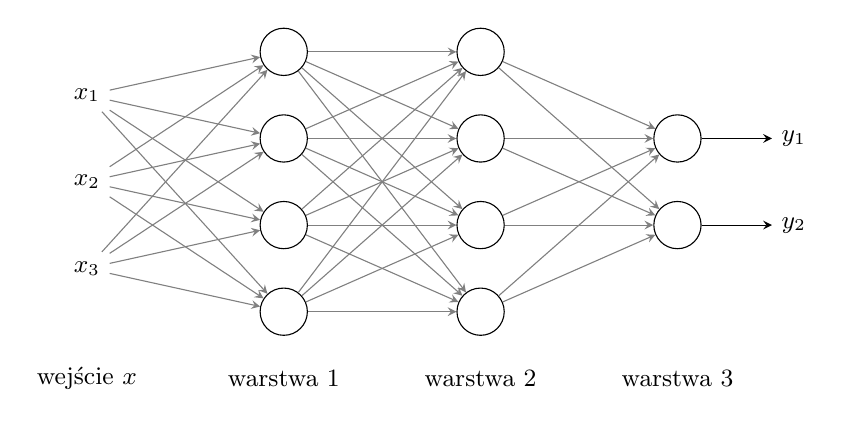
\begin{tikzpicture}[>=stealth, every node/.style={font=\small},
		neuron/.style={circle, draw, minimum size=6mm, inner sep=0pt}]
		\foreach \y [count=\i] in {1.1, 0, -1.1}
			\node (I\i) at (0, \y) {$x_{\i}$};
		\foreach \y [count=\i] in {1.65, 0.55, -0.55, -1.65}
			\node[neuron] (A\i) at (2.5, \y) {};
		\foreach \y [count=\i] in {1.65, 0.55, -0.55, -1.65}
			\node[neuron] (B\i) at (5, \y) {};
		\foreach \y [count=\i] in {0.55, -0.55}
			\node[neuron] (C\i) at (7.5, \y) {};
		\foreach \i in {1,2}
			\draw[->] (C\i) -- ++(1.2, 0) node[right] {$y_{\i}$};
		\foreach \i in {1,...,3} \foreach \j in {1,...,4}
			\draw[->, gray] (I\i) -- (A\j);
		\foreach \i in {1,...,4} \foreach \j in {1,...,4}
			\draw[->, gray] (A\i) -- (B\j);
		\foreach \i in {1,...,4} \foreach \j in {1,2}
			\draw[->, gray] (B\i) -- (C\j);
		\node at (0, -2.5) {wejście $\bm{x}$};
		\node at (2.5, -2.5) {warstwa 1};
		\node at (5, -2.5) {warstwa 2};
		\node at (7.5, -2.5) {warstwa 3};
	\end{tikzpicture}
	\caption{Sieć jednokierunkowa trójwarstwowa. Źródło: opracowanie własne na podstawie~\cite{zajdelMLP}}
	\label{fig:mlp}
\end{figure}
 
Każda warstwa $l$ ma własną macierz wag $\bm{W}^{(l)}$, wektor przesunięć $\bm{b}^{(l)}$ i~funkcję aktywacji $f^{(l)}$. Jeżeli warstwa $l$ zawiera $K_l$ neuronów, a~poprzednia $K_{l-1}$, to macierz $\bm{W}^{(l)}$ ma wymiary $K_l \times K_{l-1}$. Działanie warstwy opisuje wzór~\eqref{eq:warstwa}~\cite{zajdelMLP}:
\begin{equation}
	\bm{y}^{(l)} = f^{(l)}\left( \bm{W}^{(l)} \bm{y}^{(l-1)} + \bm{b}^{(l)} \right), \qquad \bm{y}^{(0)} = \bm{x}.
	\label{eq:warstwa}
\end{equation}
 
Złożenie zależności~\eqref{eq:warstwa} dla trzech kolejnych warstw daje wzór~\eqref{eq:mlp}, opisujący działanie całej sieci z~rysunku~\ref{fig:mlp}:
\begin{equation}
	\bm{y}^{(3)} = f^{(3)}\left( \bm{W}^{(3)} f^{(2)}\left( \bm{W}^{(2)} f^{(1)}\left( \bm{W}^{(1)} \bm{x} + \bm{b}^{(1)} \right) + \bm{b}^{(2)} \right) + \bm{b}^{(3)} \right).
	\label{eq:mlp}
\end{equation}
 
Wykazano, że sieć jednokierunkowa z~co najmniej jedną warstwą ukrytą o~nieliniowej funkcji aktywacji może z~dowolną dokładnością przybliżyć szeroką klasę funkcji ciągłych, o~ile ma wystarczającą liczbę neuronów~\cite{hornik1989}. Własność ta uzasadnia stosowanie sieci MLP do przybliżania funkcji $Q$, której postać nie jest znana.
 
\subsubsection{Funkcje aktywacji}
 
Funkcja aktywacji decyduje o~tym, jakie odwzorowania może realizować sieć. Gdyby wszystkie warstwy były liniowe, złożenie~\eqref{eq:mlp} sprowadzałoby się do pojedynczego przekształcenia liniowego, niezależnie od liczby warstw. Dlatego w~warstwach ukrytych stosuje się funkcje nieliniowe.
 
Popularną funkcją aktywacji jest ReLU, $f(z) = \max(0, z)$. Jej wadą jest zerowy gradient dla ujemnych pobudzeń: neuron, którego pobudzenie stale pozostaje ujemne, przestaje się uczyć. Zjawisko to określa się mianem ,,umierających neuronów''. Rozwiązaniem jest funkcja Leaky ReLU, opisana wzorem~\eqref{eq:leaky}, która dla ujemnych pobudzeń zachowuje niewielkie nachylenie $\lambda$~\cite{maas2013}:
\begin{equation}
	f(z) =
	\begin{cases}
		z, & z > 0, \\
		\lambda z, & z \le 0.
	\end{cases}
	\label{eq:leaky}
\end{equation}
W~bibliotece PyTorch domyślna wartość nachylenia wynosi $\lambda = 0{,}01$~\cite{pytorchLeakyReLU}. Przebieg funkcji~\eqref{eq:leaky} przedstawiono na rysunku~\ref{fig:leakyrelu}.
 
\begin{figure}[ht]
	\centering
	\begin{tikzpicture}[>=stealth, scale=0.9, every node/.style={font=\small}]
		\draw[->] (-3.2, 0) -- (3.4, 0) node[right] {$z$};
		\draw[->] (0, -1) -- (0, 3.4) node[above] {$f(z)$};
		\foreach \x in {-3, -2, -1, 1, 2, 3}
			\draw (\x, 0.07) -- (\x, -0.07) node[below] {$\x$};
		\foreach \y in {1, 2, 3}
			\draw (0.07, \y) -- (-0.07, \y) node[left] {$\y$};
		\draw[very thick] (-3, -0.3) -- (0, 0) -- (3, 3);
	\end{tikzpicture}
	\caption{Funkcja aktywacji Leaky ReLU; dla czytelności przyjęto $\lambda = 0{,}1$. Źródło: opracowanie własne}
	\label{fig:leakyrelu}
\end{figure}
 
W~warstwie wyjściowej sieci przybliżającej funkcję $Q$ stosuje się natomiast funkcję liniową, określoną wzorem~\eqref{eq:liniowa}~\cite{mnih2015}:
\begin{equation}
	f(z) = z.
	\label{eq:liniowa}
\end{equation}
Wartości funkcji $Q$ są sumami zdyskontowanych nagród, mogą więc być zarówno dodatnie, jak i~ujemne, a~ich zakres nie jest z~góry ograniczony. W~grze Snake rozważanej w~pracy zderzenie skutkuje nagrodą $-10$, zatem wartości $Q$ akcji prowadzących do kolizji są ujemne. Funkcja liniowa~\eqref{eq:liniowa} nie ogranicza zakresu wyjść, w~przeciwieństwie np. do funkcji sigmoidalnej (zakres $(0, 1)$) czy ReLU (brak wartości ujemnych).
 
\subsubsection{Uczenie sieci}
 
Uczenie sieci polega na takim doborze wszystkich jej wag i~przesunięć, zebranych w~wektor parametrów $\bm{\theta}$, aby zminimalizować funkcję straty $\mathcal{L}(\bm{\theta})$, mierzącą różnicę między odpowiedziami sieci a~wartościami docelowymi. Najczęściej stosuje się metodę spadku gradientu, w~której parametry są w~każdym kroku przesuwane w~kierunku przeciwnym do gradientu straty, zgodnie ze wzorem~\eqref{eq:gradient}~\cite{goodfellow2016}:
\begin{equation}
	\bm{\theta} \leftarrow \bm{\theta} - \eta \, \nabla_{\bm{\theta}} \mathcal{L}(\bm{\theta}),
	\label{eq:gradient}
\end{equation}
gdzie $\eta$~-- współczynnik uczenia. Gradient we wzorze~\eqref{eq:gradient} oblicza się efektywnie za pomocą algorytmu wstecznej propagacji błędu, który wyznacza pochodne straty względem parametrów kolejnych warstw, począwszy od wyjścia sieci~\cite{goodfellow2016}. W~praktyce stosuje się ulepszone warianty tej metody, takie jak optymalizator Adam, a~gradient oblicza się na podstawie niewielkich porcji danych (ang.~\emph{mini-batch}). Postać funkcji straty używanej w~algorytmie DQN omówiono w~rozdziale~\ref{sec:przeglad}, a~architekturę sieci zastosowanej w~pracy~-- w~rozdziale~\ref{sec:implementacja}.

\fi

\subsection{Gry jako środowisko badawcze}
\subsection{Przykłady zastosowań}